%%%%%%%%%%%%%%%%%%%%%%%%%%%%%%%%%%%%%%%%%
%%                                     %%
%%     LaTeX template for CCS 2019     %%
%%        abstract submissions         %%
%%                                     %%
%%          <30 March 2019>            %%
%%                                     %%
%% Author: Liu Wenyuan                 %%
%% Eamil: liuw0037@ntu.edu.sg          %%
%% Please contact author if you have   %%
%% any problem using this template     %%
%%%%%%%%%%%%%%%%%%%%%%%%%%%%%%%%%%%%%%%%%

\documentclass[11pt, a4paper]{article}
\usepackage{amsmath}
\usepackage{amsfonts}
\usepackage{amssymb}
\usepackage{graphicx}
\usepackage{hyperref}
\usepackage[top=3.17cm, bottom=2.54cm, left=2.54cm, right=2.54cm, includehead, includefoot,]{geometry}
\usepackage{authblk}
\renewcommand{\refname}{References}
%Only use following two lines if you want to use Times New Roman font
%Only work with XeLaTex or LuaLaTex
%\usepackage{fontspec}
%\setmainfont{Times New Roman}


\begin{document}
\title{\vspace{-3.0cm}\large\textbf{A multi-scalar model for system of cities}}

\author[1,2,3]{\footnotesize Juste Raimbault}
\affil[1]{\footnotesize UPS CNRS 3611 ISC-PIF, Paris, France, \url{juste.raimbault@polytechnique.edu}}
\affil[2]{\footnotesize CASA, UCL, London, UK}
\affil[3]{\footnotesize UMR CNRS 8504 G{\'e}ographie-cit{\'e}s, Paris, France}
\date{\vspace{-5ex}}

\maketitle
\thispagestyle{empty}

\noindent

% keywords
% Systems of cities
%Multi-scalar model
%Spatial interaction
%Reaction-diffusion


The modeling of urban growth is a crucial issue for the design of sustainable territorial policies, through the understanding of past urbanization processes and the forecasting of future urban trajectories. Several models have been proposed at different scales and integrating different dimensions of urban systems, such as land-use transport interaction models \cite{wegener2004land} or systems of cities models \cite{pumain2017urban}. While multi-scalar models are recognized as crucial for the study of such systems \cite{Rozenblat2018}, they remain in practice unexplored.

%At the scale of a metropolitan area, Land-use Transport Interaction models \cite{wegener2004land} are for example a privileged tool to anticipate the answer of spatial distributions of activities (mostly residential location and economic activities) to an evolution of the accessibility landscape permitted by new transportation infrastructures. At the same scale, cellular automata models of urban growth or land-use change study more generally land-use transitions with a high spatial resolution, and are mostly data-driven \cite{clarke2007decade}. At the smaller scale of the system of cities, macroscopic models of urban growth have focused on reproducing the distribution of city sizes, either through economic processes as e.g. \cite{gabaix1999zipf}, or from a geographical point of view focusing on interactions between cities \cite{favaro2011gibrat}.
%Territorial dynamics, and more particularly urban dynamics, have according to \cite{pumain1997pour} an intrinsic multi-scalar nature, with successive autonomous levels of emergence from individual microscopic agents to the mesoscopic scale of the city and the macroscopic scale of the system of cities. Furthermore, the need for sustainable territorial policies would imply the construction of multi-scalar models to take into account issues associated to each relevant scale \cite{Rozenblat2018}.
%This contribution contributes to that open question by introducing a multi-scale model of urban growth which focuses on the spatial structure of processes rather than on their multi-dimensionality. Therefore, we take into account only population variables, but both at the macroscopic scale of the system of cities in the legacy of \cite{pumain2017urban} and at the mesoscopic scale of the metropolitan area with an urban morphogenesis model. The coupling of these scales is a crucial novel feature of our model. We describe in the following stylized facts justifying the approach, describe the model, and summarize preliminary results from its exploration and calibration.

This contribution introduces a parsimonious multi-scalar model for systems of cities, based on simple dimensions (mainly populations) with stylized processes, but yielding an effective strong coupling between the metropolitan mesoscopic scale and the macroscopic scale of the system of cities. The model couples the spatial interaction model of \cite{raimbault2018indirect} for the macro scale with the reaction-diffusion model for urban form studied by \cite{raimbault2018calibration}. More precisely, urban areas viewed as a population grid are embedded into the macroscopic interaction model. To evolve populations and local urban forms, one time step consists of (i) population differences are computed by the interaction model; (ii) top-down feedback modifies parameters of mesoscopic models, given control parameters to capture typical scenarios (transit-oriented development or sprawl for diffusion, metropolization or uniformization for aggregation); (iii) local urban form are evolved with the reaction-diffusion models at a given speed conditionally to the population variations; (iv) changes in urban form influence macroscopic interaction ranges (capturing the impact of local activity on global insertion), by integrating gravity flows in the area with a squared cost function making a compromise between congestion and flows.

The model is applied on synthetic systems of cities typical of a continental range (500km, hierarchy around 1, 20 cities), with initial local population grid configurations as monocentric. Parameter space is explored with the OpenMOLE model exploration software \cite{reuillon2013openmole}, eased by the implementation of the model in scala \cite{model}. First results show a strong impact of the strong meso-macro coupling, such as for example a qualitative inversion of the behavior as a function of interaction range of macroscopic indicators trajectories when switching from a ``transit-oriented development'' scenario (negative feedback of population growth on diffusion) to a ``sprawl'' scenario (positive feedback). Similarly, mesoscopic urban form indicators are significantly influenced by the coupling process.

Further work will consist in more targeted simulation experiments, including specific exploration algorithms such as diversity search for model regimes \cite{reuillon2013openmole}, to test the model as a proof-of-concept of models for policies. Such a model can also be calibrated on real city systems and urban form trajectories, to extrapolate coupling parameters that would be difficult to obtain otherwise. Our contribution is thus a first step towards multi-scalar simulation models for systems of cities.



%\begin{figure}[!htp]
%  \centering
%  %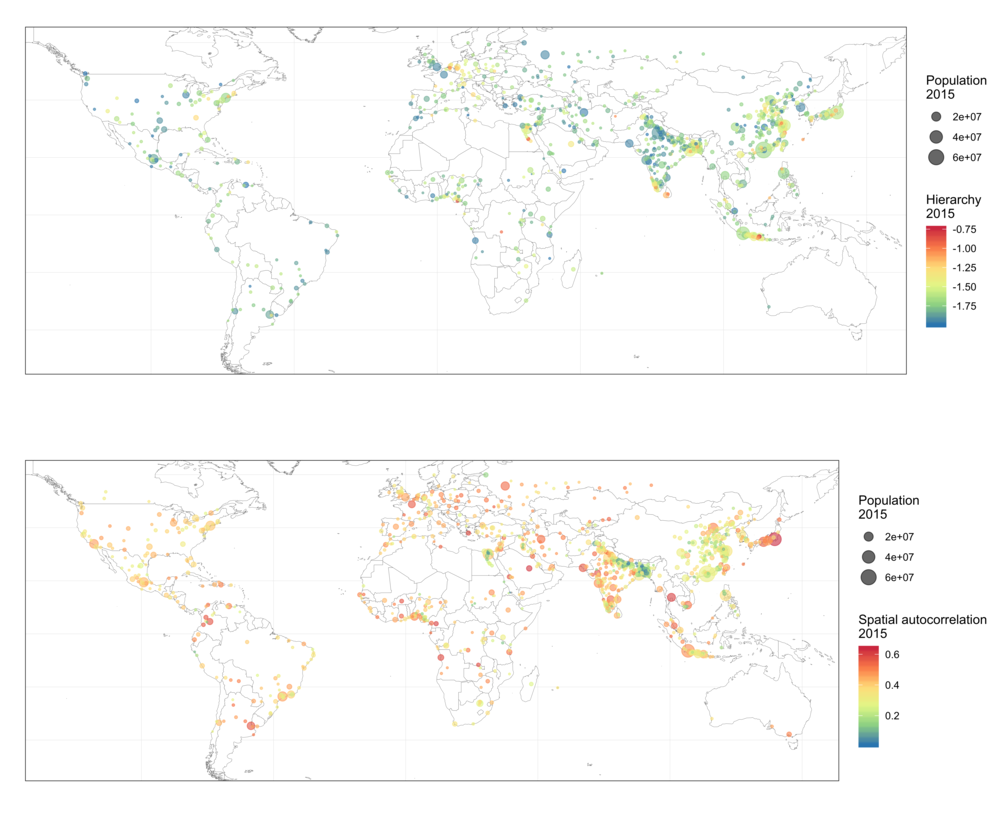
\includegraphics[width=0.6\textwidth]{Fig1.png}
%  \caption{Poincare set of the Duffing equation, for a=0.1, b=0.3}\label{fig:1}
%\end{figure}

%\noindent
%The sections for acknowledgements and references should appear at the end of the abstract (Times New Roman 11pt).

%\section*{Acknowledgements (optional)}
%The acknowledgements should be written here. Thank you for spending your time in reading the instructions. Feel free to contact us for any further information.

%\footnotesize

\bibliographystyle{unsrt}
\bibliography{biblio.bib}


\end{document} 